%!TEX root = main.tex

\section{Implementation}
In this chapter, the implementation of the main application which orchestrates everything will be presented and explained. First, the components and their functions will be briefly explained and later every main task the user can do will be explained in detail.

\subsection{Overview}
The main application is implemented in JavaScript and uses the Node.js framework. It manages all user input and executes the actions or delegates them to other components. This application is nicely packaged with Docker and runs completely on it. Only the Linux packages \texttt{docker-ce} and \texttt{docker-compose} are needed to execute this program. Figure \ref{fig:architecture} depicts all components and gives an overview of this benchmarking suite.

\begin{figure}[htp]
\begin{center}
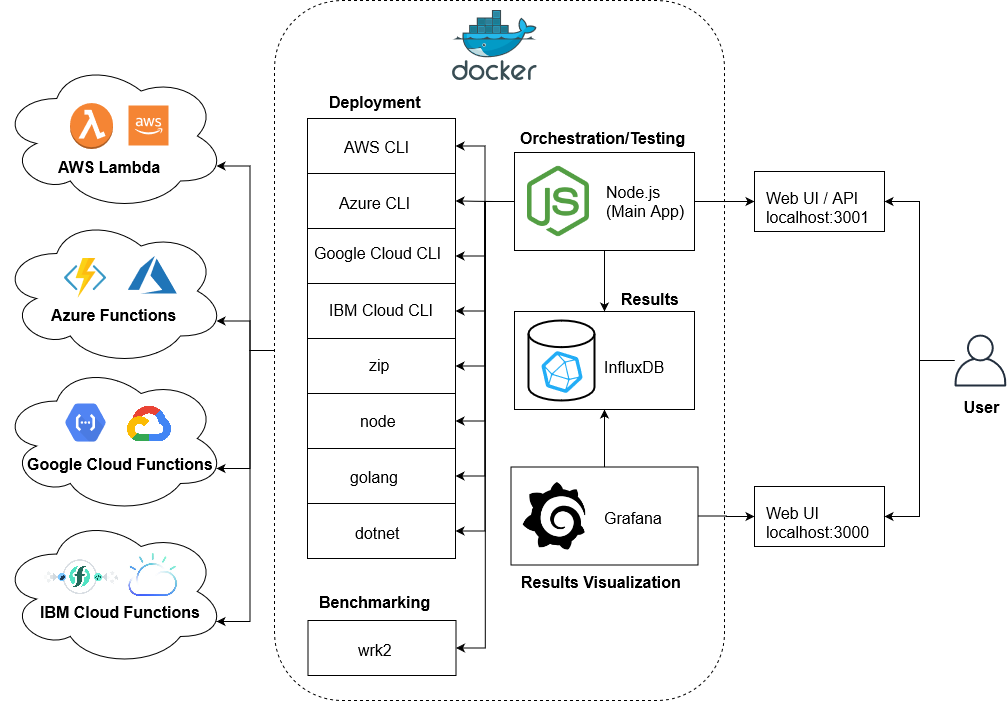
\includegraphics[width=0.77\textwidth]{bilder/main_app.png}
\captionsetup{justification=centering, labelfont=bf}
\caption[Benchmark Suite Architecture]{Benchmark Suite Architecture. Source: illustration by author}
\label{fig:architecture}
\end{center}
\end{figure}

The four clouds and their services can be seen on the left side, the involved Docker images in the middle and they ways to interact with the system can be seen on the right side. Each component will be explained step by step in the following.
\begin{itemize}
    \item \textbf{Main application:} The main application is the core of this benchmark suite and manages the four main tasks: deployment to the clouds, running simple tests, running benchmarks and calculating and estimating prices. It is available to the user through a web \gls{GUI} and also through an \gls{API}. In a first step, the user can deploy the five different tests described in section \ref{sec:tests}. Once the tests are deployed, they can be tested and benchmarked. Additionally there is a pricing calculator which calculates the cost for all four clouds either by setting the parameters manually or in regards to a previously executed test.\\
    Since the main application runs on Docker and invokes other containers which also run in Docker, the main container needs access to \texttt{/var/run/docker.sock} i.e. mounting it as volume. Otherwise a container cannot run or start another container for security and integrity reasons. This concept is called Docker-in-Docker and should generally not be used and is more of a hack than a feature. In this case it serves a simple purpose and does not implicate any issues.
    \item \textbf{InlfuxDB:} In this time series database, all the results from tests will be stored for later use in Grafana or pricing calculation.
    \item \textbf{Grafana:} Grafana is an open source tool to display, plot and monitor data stored in a database. The results gathered by the tests and stored in InfluxDB will be displayed in Grafana.
    \item \textbf{CLIs:} Each cloud provides a Docker image of their \gls{CLI} (with the exception of \gls{AWS}) to use with Docker rather than to install it on the host. Resources can be deployed, deleted and managed completely by the \gls{CLI} and no interaction on the web portal is needed. 
    \item \textbf{Runtimes (node, golang, dotnet):} In addition to the source code, a built and packaged zip file is needed for the deployment on all cloud except for Google. Therefore these three images are necessary in order to install packages and build the source code for Node.js, Go and .NET.
    \item \textbf{zip:} This simple image zips the files that need to be deployed to the clouds. Therefore there is no need to have zip installed on the machine the benchmark suite runs.
    \item \textbf{wrk2:} wrk2 is a powerful \gls{HTTP} benchmark used in this application. For simplification it is also containerized.
\end{itemize}

\subsection{Requirements}
To use this application, there are some prerequisite steps necessary. First of all, the user needs to have or create accounts on the clouds he intends to test on. This process will be not described in detail since it is straightforward to do. There is however a small guidance for each cloud provider in the documentation on GitHub.\\
Secondly, the user needs to have a Docker environment installed. This is not too difficult on Linux and described exemplary for Ubuntu 18.04 on GitHub.\\
After these steps have been completed some more manual initialization and configuration steps are required from the user. He needs to create a few Docker volumes and perform the login process for each \gls{CLI} belonging to the cloud intended to be tested.\\
As last point some free storage is required because some Docker images are quite large, in total around 5.15 GB. In addition, some free space should be reserved for the data that will be stored in the database, 1 GB should be sufficient. Table \ref{table:images} shows all images and their sizes.

\begin{table}[htp]
\centering
\captionsetup[table]{justification=centering, labelfont=bf}
\begin{tabular}{|l|l|r|}\hline
\textbf{Repository} & \textbf{Tag} & \textbf{Size} \\ \hline
bschitter/benchmark-suite-serverless-computing	&	0.1	&	358MB	\\ \hline
mikesir87/aws-cli	&	1.16.310	&	186MB	\\ \hline
google/cloud-sdk	&	274.0.1-alpine	&	287MB	\\ \hline
mcr.microsoft.com/azure-cli	&	2.0.78	&	1.04GB	\\ \hline
mcr.microsoft.com/dotnet/core/sdk	&	2.2-alpine3.9	&	1.48GB	\\ \hline
bschitter/alpine-with-zip	&	0.1	&	6.32MB	\\ \hline
bschitter/alpine-with-wrk2	&	0.1	&	232MB	\\ \hline
ibmcom/ibm-cloud-developer-tools-amd64	&	0.20.0	&	309MB	\\ \hline
golang	&	1.11-stretch	&	757MB	\\ \hline
node	&	10.16.2-alpine	&	76.4MB	\\ \hline
grafana/grafana	&	6.3.2	&	254MB	\\ \hline
influxdb	&	1.7.7-alpine	&	137MB	\\ \hline
\textbf{Total size} & & \textbf{5.15GB}\\ \hline
\end{tabular}
\caption[Docker images]{Docker images}
\label{table:images}
\end{table}

\subsection{Deployment and Cleanup}
This section will describe the deployment and the cleanup process.\\
After the application has been started, the user can use the web interface (exposed on port 3001) to take actions. The first thing he needs to do is deploy a test. The figure \ref{fig:ui} shows a screenshot of the web interface.

\begin{figure}[htp]
\begin{center}
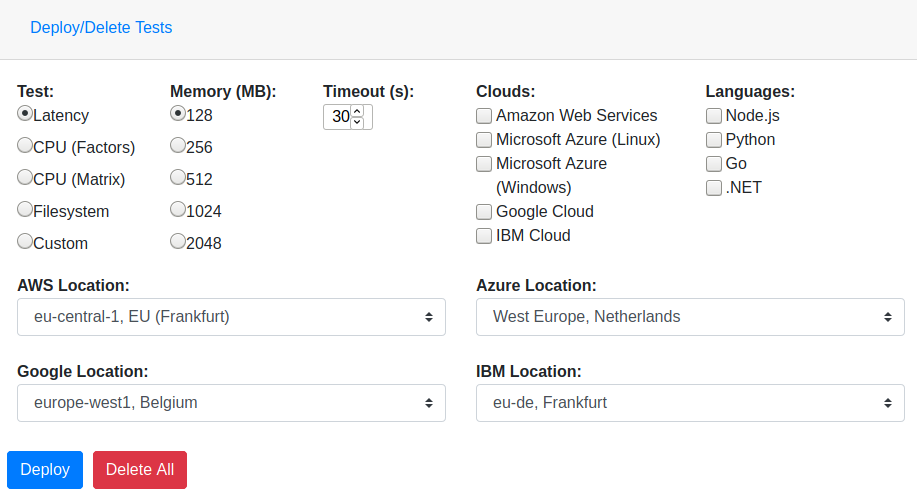
\includegraphics[width=0.7\textwidth]{bilder/ui.png}
\captionsetup{justification=centering, labelfont=bf}
\caption[Web GUI - Deploy/Delete Tests]{Web GUI - Deploy/Delete Tests, source: screenshot of the application}
\label{fig:ui}
\end{center}
\end{figure}

The following paramters can be chosen:
\begin{itemize}
    \item \textbf{Test:} The test that will be deployed (as described in section \ref{sec:tests}).
    \item \textbf{Memory:} The amount of memory the function will have available.\\ \textbf{Remark:} Not applicable for Azure as memory is assigned dynamically at a maximum of 1536 \gls{MB}.
    \item \textbf{Timeout:} The time limit after which a running function will time out.\\ \textbf{Remark:} Not applicable for Azure since it handles timeout configuration in a configuration file.
    \item \textbf{Clouds:} The cloud providers the tests will be deployed on, multiple choices possible.
    \item \textbf{Languages:} Runtimes respectively languages to deploy the function in, multiple choices possible.
    \item \textbf{Locations:} The region where the function will be deployed to.
\end{itemize}

Next the \textit{Deploy} button can be pressed and the application will initiate the deployment. On the right hand side of the web interface there will be information about the progress. The deployment process is highly parallelized (if possible) to make it as fast as possible. In the appendix \ref{chapter:flow_charts}, flow charts are illustrating the deployment and cleanup process for each cloud. For a cleanup the user can invoke the \textit{Delete All} button. Considering the cleanup is implemented very minimalist it will delete all deployed Lambda functions and \gls{API} gateways on \gls{AWS} and IBM, all resource groups with a name containing latency, factors, matrix, filesystem and custom and on Google all functions in the configured project. It should therefore be used very carefully and ideally with separate accounts only for this purpose.

\subsection{Testing}
In this section it is briefly explained how to execute a test and see its results. The test will send every five seconds a request to the functions previously deployed to see how they perform under a low, constant load. As options, a name for the test and the functions parameter can be set. The emerging result will serve as a starting point for comparison to the benchmark and optimally the function should deliver the same performance under heavy load. Figure \ref{fig:grafana} illustrates a screenshot of Grafana containing test results of a latency test in Node.js. At the top, there are three drop down menus to choose the test type, the test name (given at the start of the test) and the data points interval.

\begin{figure}[htp]
\begin{center}
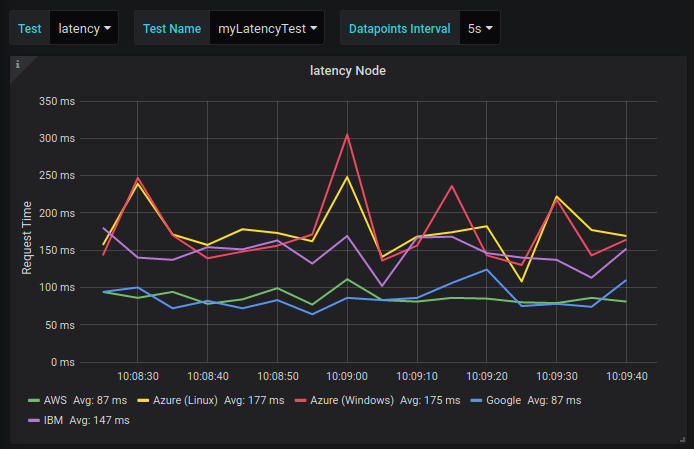
\includegraphics[width=0.7\textwidth]{bilder/grafana.png}
\captionsetup{justification=centering, labelfont=bf}
\caption[Test results in Grafana]{Test results in Grafana. Source: screenshot Grafana}
\label{fig:grafana}
\end{center}
\end{figure}

The plots can be grouped by cloud provider or by runtime. There is a predefined Grafana dashboard for both options, the user can switch depending on his interests. An example result of a general test can be seen in section \ref{sec:general_test}.


\subsection{Benchmarking}
The benchmarking part mainly relies on the wrk2 image. The parameters can be set in the web interface but they are basically just forwarded to wrk2. For the benchmark itself the user can choose the following parameters: requests per second, duration of the benchmark and the desired test to run e.g. the \gls{CPU} factors test. Afterwards the load test will start and benchmark the chosen function on each cloud and runtime it was deployed to. This process has to run sequentially otherwise the host of the benchmark suite could potentially not handle the load. After the test has completed results will be parsed and inserted into the database and can be viewed as a table in Grafana. Figure \ref{fig:benchmark_table} shows an excerpt of a result.

\begin{figure}[htp]
\begin{center}
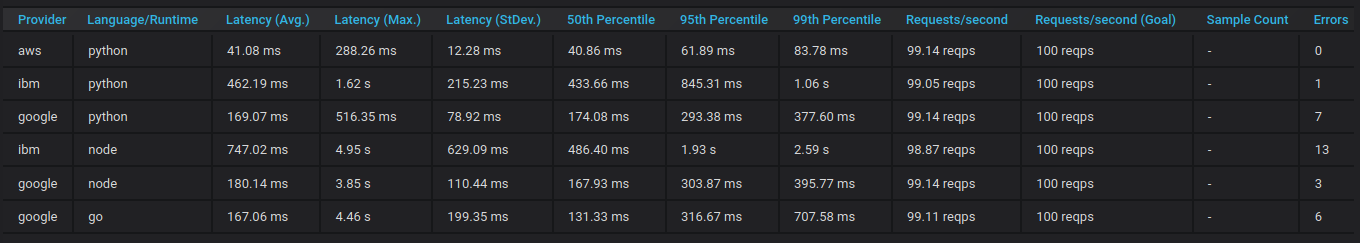
\includegraphics[width=1\textwidth]{bilder/benchmark_table.png}
\captionsetup{justification=centering, labelfont=bf}
\caption[Benchmark results in Grafana]{Benchmark results in Grafana. Source: screenshot Grafana}
\label{fig:benchmark_table}
\end{center}
\end{figure}

A more detailed test example with increasing load is discussed in section \ref{sec:loadtest}.

\subsection{Pricing}
With this component of the application one can calculate hypothetical prices by entering number of invocations, execution time per call, size of the return body and allocated memory. The prices for all clouds will be calculated and displayed in a table. The functionality is basically the same as the pricing calculators provided by the cloud providers, except here all is in one place and directly comparable.\\
Furthermore, the calculator takes the performed tests into account. One can select a previously run test, select a runtime and then one only needs to provide the estimated number of invocations per month. The calculation will happen by taking the execution time from the test results which of course can vary quite a lot between cloud providers and runtimes. This method allows a much better approach of estimated cost. In section \ref{sec:pricing} the same example will be explained and calculated for both hypothetical and with actual test results as input.